\chapter{Analyse, fortolkning og resultater}
\label{Ch:4}

I det følgende afsnit betragtes den empiri som er indsamlet i forbindelse med dette projekt.  I afsnit \vref{sec:spø} betragtes empirien som er indsamlet gennem spørgeskemaet, i afsnit \vref{sec:sam} gennemgåes den indsamlede empiri fra klassesamtalen om motivation, og kapitlet afsluttes med et afsnit \vref{sec:afv} hvor forskellige elevers skriftlige arbejde analyseres vha. TAP modellen.

\section{Spørgeskemaet}
\label{sec:spø}
Som empirisk grundlag for dette projekt er der indsamlet data via et spørgeskemaer samt fra elev afleveringer i to forskellige klasser. Alle besvarelserne på spørgeskemaet er indsamlet med SurveyXact blandt 1.g eleverne på Viborg Katedralsekole, der har været 117 ud af 349 mulige besvarelser hvilket omregnet til svarprocent er ca. \mbox{33,5 \%}. Undersøgelsen er blevet gennemført i forbindelse med praktisk eksperimentelt arbejde, hvor eleverne har besværet de fem spørgsmål umiddelbart efter det eksperimentelle arbejde og umiddelbart forud for det skriftlige arbejde. De 117 svar fordeler sig som vist på figur \vref{fig:4.1.a}. 

\begin{figure}[h!]
	\centering
	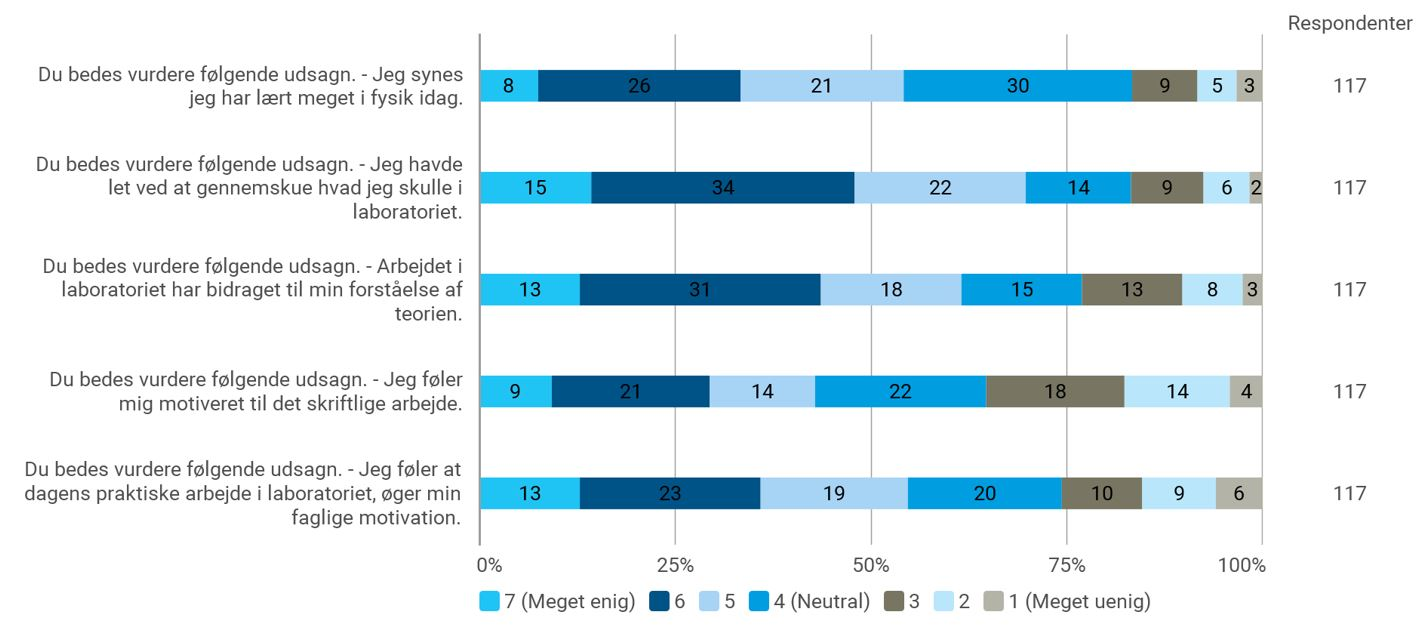
\includegraphics[width=0.9\textwidth]{Figs/Sammenlign}
	\caption[Spørgeskema resultater]{Det samlede datasæt for de fem spørgsmål med hver 117 respondenter fra en 1.g årgang på Viborg Katedralskole. Svar procenten for undersøgelsen er på omkring 33 \%. }
	\label{fig:4.1.a}
\end{figure}
Betragter man antallet af positive svar på de fem udsagn, hvor et svar regnes som positivt hvis der er svaret højere end neutral (4). Så vil det gennemsnitligt udgøre mere end 57 \% af de afgivne svar til alle fem spørgsmål (7 (meget enig) - 11,6\%, 6 - 27 \% og 5 - 18.8 \%).   Tager man elever som har en neutral holdning til de fem udsagn dækker man 77,6 \% af de adspurgte elever. Hertil kunne det anfægtes om eleverne faktisk har forstået hvad de har svaret på. Her ville man ved hjælp af Cronbach's $\alpha$ kunne afgøre om der er en intern konsistens i de afgivne svar.

\subsection*{Chronbach $\alpha$}
\begin{table}[h!]
	\centering
	\caption[Chronbach's $\alpha$ værdier]{Her ses værdier for Cronbach's $\alpha$ som mål for at teste den interne konsistens i undersøgelsen. Data som disse kan findes i en lang række artikler, men her følger vi udlægningen af \citep[Tabel 1, s. 382]{Peterson1994} hvor der er en række forskellige fortolkninger, den her anvendte tager sit udgangspunkt her og er så tilpasset.}
	\label{tbl:alpha}
	\begin{tabular}{@{ } c c @{ }}
		\toprule[2.pt]
		Værdi af Cronbach's $\alpha$ & Intern konsistens\\
		\midrule
		$0.9\leq \alpha$ 		& Fremragende\\
		$0.8\leq \alpha < 0.9$ 	& God\\
		$0.7\leq \alpha < 0.8$	& Acceptabel\\
		$0.6\leq \alpha < 0.5$	& Tvivlsom\\
		$0.5\leq \alpha < 0.6$ 	& Dårlig\\
		$\alpha < 0.5$			& Uacceptabel\\
		\bottomrule[2pt]
	\end{tabular}
\end{table}
Cronbach's  $\alpha$ er beregnet på følgende vis: 
\begin{equation}\label{eq:alpha}
	\alpha = \left(\frac{k}{k-1}\right)\cdot \left(1-\sum_{i=1}^{k} \frac{\sigma^{\phantom{i}2}_{i}}{\sigma^{\phantom{s}2}_{s}}\right)
\end{equation}
hvor $k$ er altallet af målinger i undersøgelsen, $\sigma^{\phantom{i}2}_{i}$ er variansen af den i'te måling, mens $\sigma^{\phantom{s}2}_{s}$ er variansen for hele undersøgelsen, jf \cite[s.382]{Peterson1994}. For de indsamlede data i spørgeskemaet er Cronbach's $\alpha$ beregnet til 0.91, hvilket baseret på skalaen i tabel \vref{tbl:alpha} betyder at der er en fremragende intern konsistens i undersøgelsen. Hvilket igen betyder at elevernes svar er konsistente gennem alle spørgsmålene. 

På baggrund af de 117 besvarelser af spørgeskemaet er det muligt at beregne en Chronbach $\alpha$ for datasættet. Her findes værdien for Chronbach $\alpha$ til 0,91 hvilket tyder på at der er en virkelig god intern konsistens i undersøgelsen jf. tabel \tbref{alpha}. Det tyder også på at eleverne har forstået de fem spørgsmål som de er blevet bedt om at svarer på.  Generelt ser det ud til at hvis en elev svarer lavt, kategori 1 og 2, på spørgsmål et så svarer den pågældende elev lavt på alle fem spørgsmål. Ligeledes hvis en elev svarer højt, kategori 6 og 7, så svarer de generelt over middel på alle spørgsmålene. Med andre ord er eleverne baseret på deres selvevaluering enten motiverede eller også mangler de motiation i det praktiske arbejde.

\subsection*{Opsamling på spørgeskemaet}
Det er altså tydeligt med udgangspunkt i den empiri der er indsamlet i forbindelse med spørgeskema undersøgelsen at eleverne generelt føler at de lære noget af det praktiske arbejde, samt at de kan gennemskue hvad de skal i laboratoriet, men det halter stadig med at kunne motivere eleverne til det skriftlige arbejde, som det fremgår af figur \firef{4.1.a}.
Kigger man på nogle af de kommentarer som eleverne har givet finder man udsage som:
\begin{quote}
	``[\ldots]\emph{Jeg har i dette forløb om ideal gasser, været lidt udfordret pga at vi ikke har fået noget teori forklaret på tavlen. Dette gjorde mig en del umotiveret.}[\ldots]''\vspace{-15pt}
\begin{flushright}
	Elevkommentar fra spørgeskemaet
\end{flushright}
\end{quote}
Dette til trods for at den pågældende elev har vurderet alle fem spørgsmål højt eller meget højt. Så der er en klar udfordring i hvorledes resultaterne så skal fortolkes, når eleverne vurderer udsagnene på en måde og efterfølgende skriver noget anden end det deres vurdering umiddelbart ser ud til. Det er dog tydeligt at denne pågældende elev er udfordret af \ib{}-tilgangen til undervisningen. Baseret på kommentaren kan det tolkes at denne elev har været en del af test klassen. Om end en af de store udfordringer i forbindelse med denne undersøgelse er at det ikke er muligt at trække de elever ud som har været i test gruppen og se på deres resultater uafhængigt af de øvrige 1.g elever, da spørgeskemaet har været gennemført anonymt for at opnå så pålidelige og reelle svar fra eleverene. Det er dermed kun muligt at hente information om eleverne er en del af test gruppen såfremt de som i udsagnet ovenfor klart giver udtryk for at de tilhører testgruppen. den overordnede konklusion ser ud til at være at eleverne generelt motiveres ved at lave eksperimenter i fysikfaget men at det halter med at motivere eleverne til det skriftlige arbejde i fysikfaget.  

\section{Samtale om motivation for skriftlighed}
\label{sec:sam}
I forbindelse med undervisningen i fysik faget i klassen 1.y på Viborg Katedralskole blev der gennemført et dialog med klassen med fokus på emnet motivation. Her definerede klassen begrebet motivation som ``Lysten til at gøre noget''. På baggrund af denne definition af begrebet førte dialogen over til hhv. ydre og indre motivation og årsager til at man kan finde ydre motivation og hvordan man i undervisningsrummet kan nå den ydre motivation men kan have svært ved at påvirke elevernes indre motivation for faget, jf. \citep{Buhl2010}. I forbindelse med ydre og indre motivation sætter eleverne de samme benævnelser på de to motivations begreber som man kan finde i litteraturen. Efterfølgende snakkede klassen om hvad begrebet faglig motivation dækker over. Her kom en version af den oprindelige definition af begrebet som lød ``Lysten til at lære noget''. Hertil spurgte undervisere hvad vil det sige at lære noget? Til dette kom der mange bud, blandt andet at man skulle kunne bruge sine tillærte kompetencer til noget. Eller at man kunne huske det man havde lært tidligere. Til spørgsmålet om hvorvidt eleverne blev motiveret mest af mundtligt eller skriftligt arbejde var det entydige svar, at eleverne blev klart mest motiveret af mundtligt arbejde. Der var i høj grad tale om en ydre motivation hvor eleverne fremhævede feedback og respons fra klassen og underviserne som det mest motiverende. Eleverne mente ligeledes at de havde lettere ved at forholde sig til den feedback de fik mundtligt. Sluttelig drejede samtalen over på hvordan man ville kunne øge motivationen for det skriftlige arbejde. Her pegede eleverne på at de i højere grad ønskede mundtlig feedback med fokuspunkter end skriftlig feedback med fokuspunkter for det ville gøre at de kunne spørge ind til dele af den modtagne feedback. De pegede også på at de mente at opgaveskrivning i mindre skridt ville være mere optimalt, samt en klarer instrukser af hvad der skulle være en del af opgaven. Eleverne ønskede også et skrive modul i umiddelbar forlængelse af deres eksperimentelle moduler. Samt mere tid til den eksperimentelle del af undersøgelserne.

\subsection*{Opsamling på samtalen}
Eleverne er i den beskrevne samtale inde at røre ved noget så fundementalt som dannelse nemlig evnen til at kunne binge sin faglighed i spil uden for klasserummets vægge. I denne kontekst er det åbentlyst at eleverne udelukkende opfatter rapporter og journaler som skriftligt arbejde og altså ikke regneopgaver udført i timerne som en del af den daglige undervisning, hvor eleverne træner færdigheder og problemløsningskompencer. Forholder man sig til de tiltag som eleverne stiller op som faktorer som kunne øge deres skriftlige motivation så er der flere af tingene som giver god mening, fx.
\begin{itemize}
	\item Opgaveskrivning i mindre bidder \vspace{-15pt}
	\item Skrive moduler umiddelbart efter eksperimentet\vspace{-15pt}
	\item Mundtlig feedback
\end{itemize}
Opgaveskrivning i mindre bidder giver mening i forhold til at klæde eleverne på til bedst muligt at løse denne opgave. Dette kunne man også udnytte i forhold til at anvende et undervisningsmodul i forbindelse med enhver øvelse der laves således at det kan kvalificeres for eleverne hvordan man bygger de enkelte dele af en rapport/journal op. 
Pinden med mundtlig feedback giver mulighed for at eleverne kan stille spørgsmål til den feedback de får men det kan på samme tid problematiseres at eleverne her vil få problemer med at fastholde deres fokuspunkt til næste aflevering, hvis dette udelukkende overdrages mundtligt. Man kunne derfor overveje om det ville give mening med at give eleverne mundtlig feedback via vodcasts fx med Screencast'O'Matic herved kan man også se hvor mange gange eleverne ser casten.

Man kan undre sig over at eleverne ikke føler at de er klar over hvad der skal være med i rapporten/journalen når de har fået både mundtlig og skriflig information herom samtidig med at de har haft tid i skolen til at arbejde med afleveringen. Dette kunne igen måske afhjælpes ved at opbygge skrivningen i mindre dele med særligt fokus på enkelt dele af skrive processen.

\section{Afleveringer}
\label{sec:afv}
Til at belyse den sidste del af denne undersøgelse nemlig spørgsmålet om hvorvidt den skriftlige kompetence udvikles gennem anvendelsen af \ib{} og SWH i samspil. Anvendes elev afleveringer, som analyseres efter Toulmins Argumentations Princip (TAP). I denne del af empirien analyseres fire afleveringer fra klassen 1.y hvor der udtages to tilfældigt valgte afleveringer fra den første rapport som eleverne afleverede og to fra den aflevering eleverne afleverede lige inden påske. På samme vis er der udtaget to gange to afleveringer fra en anden 1.g klasse på Viborg Katedralskole.
De otte afleveringer er fordelt på følgende måde hvor elev 1 og elev 2 er fra kontrolgruppen: 
\begin{enumerate}
	\item[Elev 1] 1.e - Nyttevirkning af elkedel og kaffemaskine samt Bestemmelse af bølgelængde for laserlys\vspace{-15pt}
	\item[Elev 2] 1.e - Nyttevirkning af elkedel og kaffemaskine samt Bestemmelse af bølgelængde for laserlys\vspace{-15pt}
	\item[Elev 3] 1.y - Undersøgelse af fænomenet gnidning og Undersøgelse fænomenet diffraktion\vspace{-15pt}
	\item[Elev 4] 1.y - Undersøgelse af fænomenet gnidning og Undersøgelse fænomenet diffraktion
\end{enumerate}

\subsection*{Nyttevirkning af elkedel og kaffemaskine}
Når man ser på de første to rapporter fra hhv. elev 1 og elev 2 så er det svært at indetificere det skema som er beskrevet på figur \firef{tou}. Der er i høj grad tale om en rapport som er skrevet med ført hånd af den vejledning som eleverne har fået på forhånd. Det har været helt klart for eleverne hvilket resultat de forventedes at opnå med øvelsen. Det tætteste vi kommer på en egentlig påstand er følgende pasus
\begin{quote}
	``[\ldots]\emph{$\Delta$Enytte er den energi, som udnyttes til opvarmning af vandet. Når vi har en mængde vand med massen m, kan denne energi beregnes ved hjælp af formlen;
	\begin{equation*}
	\Delta Enytte = m\cdot c\cdot \Delta T
	\end{equation*}
	hvor $c$ er den specifikke varmekapacitet (varmefylde) for vandet}[\ldots]''
\end{quote}
Problemet her er at denne påstand ikke er funderet i data så det er i virkeligheden det facit som eleven burde nå frem til men hvordan undersøges dette? Endvidere er dette uddraget fra den teoretiske del af vejledningen jf. appenix \vref{app:B}. For både elev 1 og elev 2 er data her forstået som tal tastet ind i et skema som har været tegnet op på forhånd. Eleverne har dermed blot skulle taste tydeligt definerede værdier ind i skemaet, i passende allerede angivne enheder. Data er for de to grupper ikke overraskende meget lig hinanden. I forhold til at skabe evidens for den påstand som fremgår af tekstuddraget her over, så forbliver evidensen her blot udregninger med de allerede givne formler. Sluttelig er rygdækningen her den første del af rapporten hvori teorien gennemgåes, dog med det lille twist at dette afsnit mere eller mindre kommer fra øvelsesvejledningen. Betragtes vejledningen til denne øvelse, se appendix \vref{app:B}, er det tydeligt at denne ikke overlader meget til fantasien og til at eleverne frit kan eksperimentere i laboratoriet. Vejledningen strukturere arbejdet såvel som databehandlingen for eleverne. Det er derfor meget svært at ende ud med forskellige slutprodukter samt at fordre forundring og kreativitet blandt eleverne dette ses også tydeligt på de to produkter som eleverne har afleveret. 
Anvendes TAP modellen finder man et fint skema med de opsamlede data jf. skemaet \tbref{data.forsøg1}. Her er alt systematiseret og eleverne skal for at kunne fylde det hele ud foretage relevante beregninger. 
Men der udformes på intet tidspunkt en påstand på baggrund af de foreliggende data og der søges ej heller evidens, grundet den manglende påstand. Dermed forbliver arbejdet en anelse fremmet overfor den måde man argumentere videnskabeligt for de valg man foretager undervejs i det praktiske arbejde. 

\subsection*{Bestemmelse af bølgelængden for laserlys}
I denne øvelse skal eleverne undersøge fænomenet diffraktion af laserlys ved passage af et optisk gitter. I ligesom i vejledningen fra undersøgelsen beskrevet ovenfor så overlades ikke meget til eleverne her. Dog skal eleverne denne gang selv formulere formålet med øvelsen  samt teoriafsnittet, som dog har nogle mindste krav til undersøgelsen. I denne vejledning er der som i den første vejlednign et fint skema som eleverne kan bruge til at notere data i. og databehandlingen udføres igen med ført hånd således at eleverne udfører de væsentlige undersøgelser bl.a. skrives følgende i vejledningen:
\begin{quote}
	``[\ldots]\emph{Hvis $n$ og $\lambda$ er kontstante (og det er de i vores forsøg), så er $\sin(\theta)$ en lineær funktion af $n$, med hældningskoefficienten $\lambda\per d$ og b-værdi på 0 (svarende til $y = a\cdot x + 0$).}'[\ldots]'
\end{quote}
Dette kunne have været baggrund for en rigtig god påstand for eleverne at komme med på baggrund af deres datasæt. Men igen anvendes data kun i ringe omfang til at sige noget om sammenhænge. Dog fremstilles evidensen for den påstand som er indlejret i ovenstående citat fra vejledningen. 
\begin{figure}[h!]
	\centering
	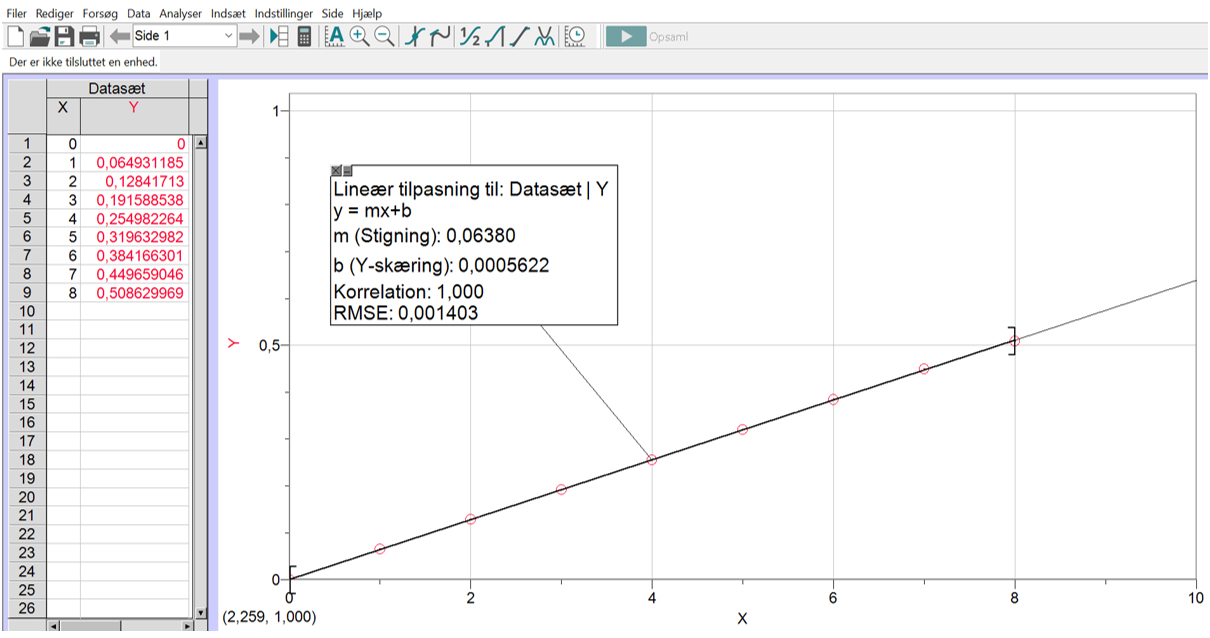
\includegraphics[width=\textwidth]{Figs/EviHan}
	\caption[Elev produktion 1]{Eksempel på evidens hentet fra afleveringen om bestemmelse af bølgelængden for laserlys fra elev 1}
	\label{fig:elev1}
\end{figure}
Denne graf, se figur \firef{elev1} er lavet af både elev 1 og elev 2 som det er beskrevet i vejledningen, og fælles for eleverne er at denne ikke anvendes yderligere i forhold til at be- eller afkræfte teorien, der er i spil. Dette kan skyldes at der ikke er tale om at validere en påstand. Eleverne kommer hermed ikke til at reflektere over det de har undersøgt - man kunne overveje at have omformuleret ovenstående citat således at det kom til at lyde noget i retning af 
\begin{center}
``Undersøg sammenhængen mellem $\sin(\theta)$ og $n$.''
\end{center}
Det ville også give eleverne en bedre mulighed for at komme helt rundt i deres faglige argumentation, med et særligt fokus på TAP modellen da alle skolens klasser er blevet introduceret til Toulmins argumentations princip i forbindelse med et internt  argumentationsprojekt på Viborg Katedralskole. Endvidere har man ikke givet eleverne facit, nemlig at sammenhængen er lineær og eleverne skal altså finde en måde at afgøre hvad der skal ske med data i forhold til at uddrage information fra dem, samtidig tvinges de tilbage i det teoretiske fundament for øvelsen for at søge rygdækning for den påstand de ville fremkomme med i forbindelse med denne undersøgelse. 

\subsection*{Undersøgelse af fænomenet gnidning}
Til dette eksperiment havde eleverne ingen vejledning, derimod blev der brugt et modul på at udforske forforståelsen af fænomenet gnidning, samt at finde ud af hvad man kunne undersøge i laboratoriet omkring fænomenet gnidning. Her udviklede eleverne i grupper deres egne undersøgelsesspørgsmål og definerede hvordan de havde tænkt sig at undersøge netop dette spørgsmål i laboratoriet. Herunder hvilket laboratorie udstyr de havde brug for. Grupperne hvori elev 3 og elev 4 var kom frem til følgende undersøgelsesspørgsmål.
\begin{itemize}
	\item[{\bfseries Elev 3}] Er en overflades $\mu$-indeks altid det samme uanset objektets masse?\vspace{-15pt}
	\item[{\bfseries Elev 3}] Er et objekts $\mu$-indeks det samme på alle af de valgte overflader?\vspace{-15pt}
	\item[{\bfseries Elev 4}] Er der en sammenhæng mellem massen af legemet og størrelsen af gnidningskræften?
\end{itemize}
Efter en samtale med gruppen hvori elev 3 befandt sig stod det klart at de med ordet $\mu$-indeks mente gnidningskoefficient. Elevgruppen med elev 3 valgte altså to undersøgelsesspørgsmål hvor De i alt foretog 12 målinger med fire forskellige masser på tre forskellige underlag. Dette gav dem et fint datasæt. Med udgangspunkt i deres datasæt kunne de udlede følgende påstande. 
\begin{enumerate}
	\item Gnidningskoefficientet er tilnærmelsesvis uafhængig af objektets masse.\vspace{-15pt}
	\item Gnidningskoefficientet er stærkt afhængig af underlaget.
\end{enumerate}
Med udgangspunkt i deres data og deres påstand påbegynder gruppen efterfølgende at lave en graf som kan danne evidens for deres påstand. Som evidens for den for deres anden påstand har gruppen af elever frembragt følgende figur \firef{evidens.alma}.
\begin{figure}[h!]
	\centering
	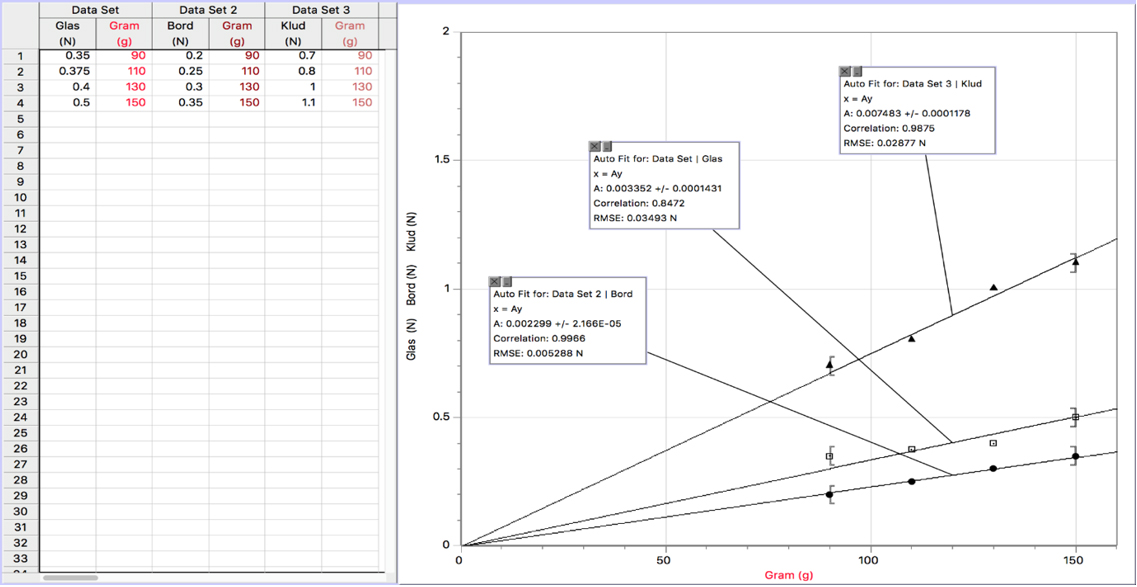
\includegraphics[width=\textwidth]{Figs/EviAlm}
	\caption[Elev produktion 2]{Evidens til at understøtte de påstande som er uddraget af data. Her er gnidning mod bord markeret med cirkler, mod glas med firkanter og mod en klud med trekanter}
	\label{fig:evidens.alma}
\end{figure}

Fra tabellen i venstre side af figur \firef{evidens.alma} fremgår det at variation af massen kun har en lille eller slet ingen betydning for gnidningskoefficienten mens variation af underlaget har en enorm betydning for gnidningskoefficienten som det klart fremgår af det grafiske evidens i figurens højre panel, som eleverne også fremhæver. 
Den sidste del af TAP-modellen som det bør tjekkes om denne aflevering lever op til er kravet om rygdækning, her skal rygdækningen søges i afleveringens teori afsnit hvor eleverne har hentet inspiration i deres fysik bog \citep{Benoni2010} hvori eleverne har fundet inspiration i kapitlet om kræfter til en beskrivelse af gnidningskræften.

Gruppen hvor elev 4 er medlem er kommet frem til en lignende konklusion og med evidens der minder om det som er beskrevet herover. Deres opbygning af undersøgelsen er også som herover. Hvorfor der ikke er nogen mening i at gennemgå det i stor detalje. 

\subsection*{Undersøgelse af fænomentet diffraktion}
I denne undersøgelse er eleverne 3 og 4 kommet på forskellige undersøgelser. Når man betragter de afleveringer som eleverne har lavet i forbindelse med denne undersøgelse så er det tydeligt at de er faldet ned i et rapport design som minder mere om den klassiske rapport skabelon som vist i tabel \tbref{2.1}. Dette til trods for at underviseren havde gjort det klart for eleverne at de skulle huske på hvad de havde lært om skriftlighed. Deres klassiske afleveringer var dog ikke totalt identiske med den klassiske rapport skabelon fx havde ingen af rapporterne et afsnit om formålet med undersøgelsen i stedet havde de begge en hypotese hvori de beskrev de forventninger de havde til undersøgelsen. I forbindelse med hypotesen var der de undersøgelsesspørgsmål som eleverne havde udarbejdet i grupperne forud for eksperimentet. Herefter er det fælles for rapporterne at de efter at have beskrevet en fremgangsmåde og deres data og observationer glemmer at udfærdige påstande jf. Toulmins Argumentations Princip, som efterfølgende kan eftervises med den evidens der kan skabes ud fra den indsamlede empiri. Begge elevgrupper søger dog at skabe en form for evidens for deres undersøgelse, men den forbliver ufokuseret i forhold til det de faktisk kan uddrage af den indsamlede empiri.

For begge grupper når de ikke helt i mål med det de har sat sig for at undersøge. Gruppen med elev 3 i havde sat sig for at undersøge om fabrikatens påtrykte gitterkonstant faktisk passede med hvad man kunne bestemme den til i laboratoriet. Hvorimod gruppen med elev 4 satte sig for at undersøge sammenhængen mellem antallet af ordner og interferenspletternes afstand fra den centrale orden. 

Når man som underviser betragter gruppernes data er det helt tydeligt at der er gået noget helt galt. I tilfældet med gruppe tre er der blevet byttet om på nogle af de målte størrelser og dette kommenteres også i forbindelde med refleksionerne over eksperimentet. Dette betyder også at gruppen på igen måde ville kunne skabe evidens for noget, grundet enorme usikkerheder jf. de grove notations fejl. For gruppen med elev 4 blev det til følgende empiriske data, se figur \firef{evidens.jacob}.

\begin{figure}[h!]
	\centering
	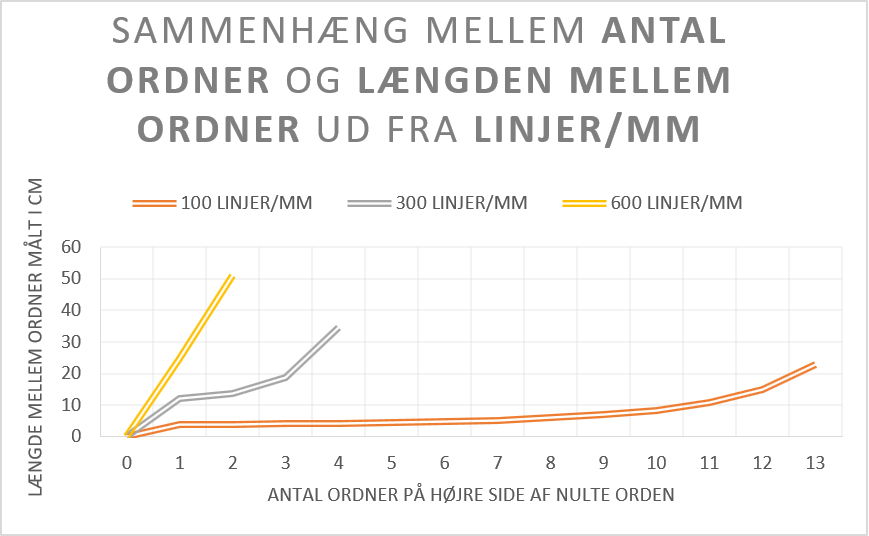
\includegraphics[width=\textwidth]{Figs/EviJacob}
	\caption[Elev produktion 3]{Her ses den eviden som gruppen med elev nummer 4 frembragte i et forsøg på at understøtte deres hypotese om linearitet mellem }
	\label{fig:evidens.jacob}
\end{figure}

Her plotter eleverne antallet af interferenspletter langs førsteaksen mens de plotter afstanden mellem ordnerne på anden aksen. Heraf fremgår det klart at der ikke er nogen form for linearitet mellem antallet af ordner og afstanden mellem ordnerne. Overraskende nok passer den viste evidens med den sammenhæng som eleverne burde komme frem til. Gruppen opsummerer også på deres graf og påpeger at linjen på figur \firef{evidens.jacob} som svarer til 600 linjer pr mm, ser ud til at være proportional men at den er dannet ud fra to punkter og at man derfor ikke kan sige noget klart. Hvilket er en helt korrekt slutning.
Udfordringen for eleverne her har været at de ikke nødvendigvis har de fornødne matematiske værktøjer til at analyserer denne situation og forstå data således at de kan se om det passer med teorien, da der her indgår flere trigonometriske funktioner, en lidt mere uddybende analyse af problemet vedrørende denne graf kan findes beskrevet i appendix \vref{app:C}. Det er en klar udfordring som er forbundet med denne arbejdsform hvor eleverne jf \ib-metoden selv i højere grad driver værket. 

På det refleksive plan er både gruppen med elev 3 og elev 4 meget langt i deres læreproces fx skriver gruppen med elev 3 om resultaterne af deres eksperiment;
\begin{quote}
``[\ldots]\emph{Vores forsøg understøtter teorien om  det optiske gitter. Da vi sendte laserens stråle igennem et optisk gitter opstod der et interferensmønster, og det understøtter altså teorien om ringbølger, konstruktiv- og destruktivinterferens. I forhold til vores undersøgelsesspørgsmål virker det til, at gitterkonstantens afvigelse fra fabrikantens dekleration til vores egne beregninger er ude af proportion og uden sammenhæng mellem gitrene}[\ldots]''
\end{quote}
Denne type af refleksioner over egne resultater finder man ikke i rapporterne hos de elever som blindt har fulgt en kogebogs vejledning. Eleverne i gruppen med elev 3 fortsætter deres refleksioner over hvad der kan være gået galt, med en perspektivering som peger i retning af hvordan man kunne forbedre eksperimentet. Herunder en undersøgelse af hvad det ville betyde for resultaterne hvis man måler 1 \centi\meter{} forkert med målebåndet, her er deres konklusion at det med deres data kan betyde afvigelser på op til 20 \%. Det er meget atypisk for elever på dette niveau, at man reflektere over hvorfor man får resultater som afviger så meget fra hvad man havde forventet at få. Sammenligner man med den første rapport er det også tydeligt at eleverne har udviklet sig i form af deres måde at undre sig på og i deres måder at forholde sig kritisk til de resultater de havde forventet at få. Det er altså klart at kombinationen af undervisning efter \ib-tanken og skriftlighed efter SWH-metoden har givet eleverne et kritisk blik for hvad de får ud af eksperimenterne og med dette krittiske blik undersøger de mulige fejlkilder og deres indvikrning på resultaterne i undersøgelsen. 

\section{Opsummering}
Når man betragter den klassiske rapport over for SWH rapporten, begge beskrevet i tabel \tbref{2.1}. Så er de afleveringer som indleveres af elever som er skrevet efter SWH metoden langt mere velreflekterede og der er meget bedre sammenhæng mellem det eleverne gør i laboratoriet og det udbytte de får af deres eksperimentelle arbejde. Endvidere lader det til at elevernes engagement stiger da de selv er med til at bestemme hvilken retning deres eksperiment skal bevæge sig i.  

%\begin{figure}[h!]
%	\centering
%	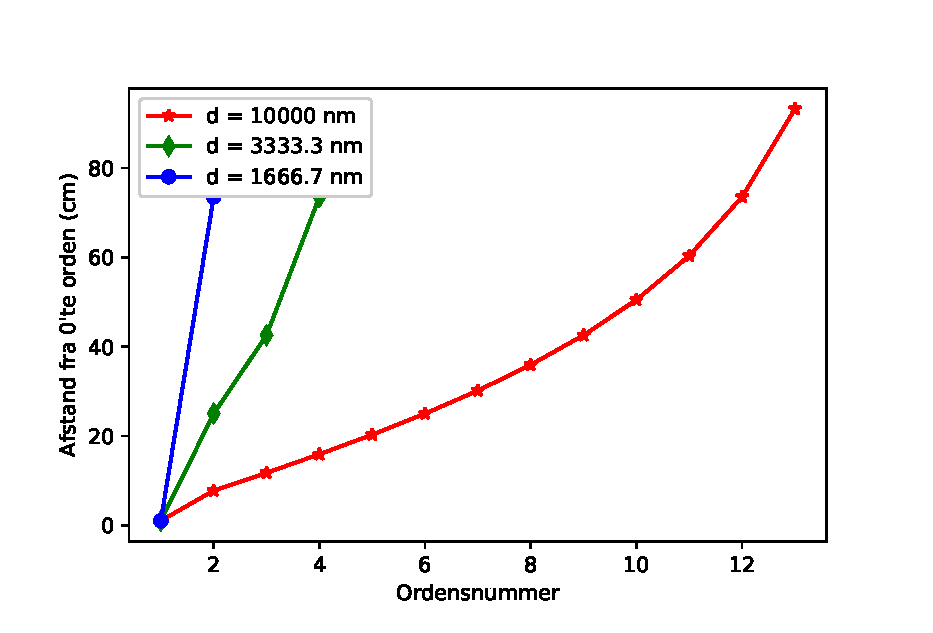
\includegraphics[width=.75\textwidth]{Figs/test}
%\end{figure}
